\subsection{棱台、圆台的体积}\label{subsec:2-10}
\begin{enhancedline}

我们已知,棱台、圆台分别是棱锥、圆锥用平行于底面的平面截去一个锥体得到的。
因此,台体的体积可以用两个锥体的差来计算。

\begin{figure}[htbp]
    \centering
    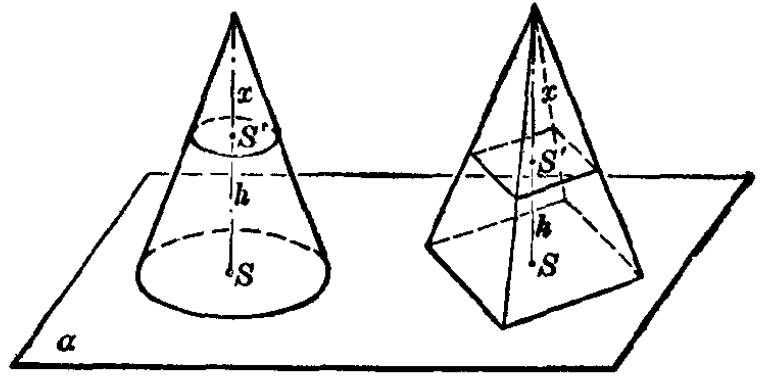
\includegraphics[width=10cm]{../pic/ltjh-ch2-67.png}
    \caption{}\label{fig:ltjh-2-67}
\end{figure}

设任意台体(棱台或圆台)的上、下底面的面积分别是 $S'$、$S$,高是 $h$。
截得台体时去掉的锥体的高是 $x$,去掉的锥体和原来的锥体的体积分别是 $V'$、$V$(图 \ref{fig:ltjh-2-67})。这时,
$$ V' = \exdfrac{1}{3} S'x \douhao  V = \exdfrac{1}{3} S (h + x) \douhao $$
所以台体的体积
$$ V_\text{台体} = V - V' = \exdfrac{1}{3} S (h + x) - \exdfrac{1}{3} S'x = \exdfrac{1}{3} [Sh + (S - S')x] \juhao $$
因为台体上、下底面相似,所以
\begin{align*}
    & \dfrac{S'}{S} = \dfrac{x^2}{(h + x)^2} \douhao \quad \dfrac{\sqrt{S'}}{\sqrt{S}} = \dfrac{x}{h + x} \douhao \\
    & x = \dfrac{\sqrt{S'} h}{\sqrt{S} - \sqrt{S'}} \juhao
\end{align*}
代入上式,得
\begin{align*}
    V_\text{台体} &= \exdfrac{1}{3}h \left[S + (S - S') \dfrac{\sqrt{S'}}{\sqrt{S} - \sqrt{S'}}\right] \\
        &= \exdfrac{1}{3}h [S + \sqrt{S'} (\sqrt{S} + \sqrt{S'})] \\
        &= \exdfrac{1}{3}h (S + \sqrt{SS'} + S') \juhao
\end{align*}

由此我们得到下面的定理:

\begin{dingli}[定理][dl:taiti-tj]
    如果台体(棱台、圆台)的上、下底面的面积分别是 $\bm{S'}$、$\bm{S}$,高是 $\bm{h}$,那么它的体积是
    \begin{center}
        \framebox[16em]{$\bm{V_\text{台体} = \exdfrac{1}{3}h (S + \sqrt{SS'} + S')}$。}
    \end{center}
\end{dingli}

\begin{tuilun}[推论][tl:taiti-tj]
    如果圆台的上、下底面半径分别是 $\bm{r'}$、$\bm{r}$,高是 $\bm{h}$,那么它的体积是
    \begin{center}
        \framebox[16em]{$\bm{V_\text{圆台} = \exdfrac{1}{3} \pi h (r^2 + rr' + r'\,^2)}$。}
    \end{center}
\end{tuilun}

最后,我们注意到,在台体的体积公式中,
如果设 $S' = S$,就得到柱体的体积公式 $V_\text{柱体} = Sh$;
如果设 $S' = 0$,就得到锥体的体积公式 $V_\text{锥体} = \exdfrac{1}{3} Sh$。

这样,柱体、锥体、台体的体积公式之间的关系,可表示如下图:

\begin{figure}[htbp]
    \centering
    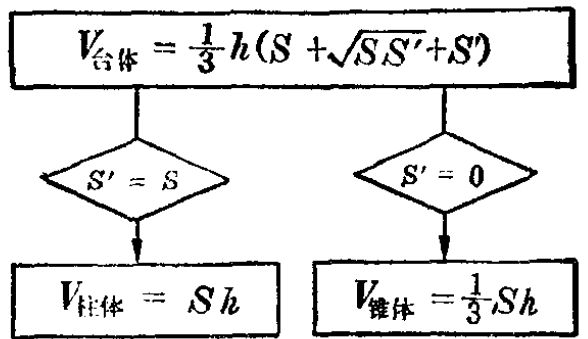
\includegraphics[width=8cm]{../pic/ltjh-ch2-subsec10-gsgx.png}
\end{figure}

\liti[0] 有一个正四棱台形油槽,可以装煤油 190 升,假如它的两底面边长分别等于 60 cm 和 $40\;\limi$。 求它的深度。

\jie $\because$ 上底面面积 $S' = 40^2 = 1600$,

        \hspace{2.5em}  下底面面积 $S  = 60^2 = 3600$,

        \hspace{2.5em} $\sqrt{S \cdot S'} = \sqrt{40^2 \times 60^2} = 2400$,

$\therefore$ \quad $V = \exdfrac{1}{3}h (3600 + 2400 + 1600) = \exdfrac{7600}{3}h$。

由已知 $V = 190 \text{升} = 190000 \;\lflm$,

$\therefore$ \quad $h = \exdfrac{3 \times 190000}{7600} = 75\;(\limi)$。

答:油槽深度是 75 cm。


\begin{lianxi}

已知上、下底面边长分别是 $a$、$b$,高是 $h$。求下列正棱台的体积:
(1)正四棱台; (2)正六棱台。

\end{lianxi}

\end{enhancedline}

